%=======================================================================
% Copyright (c) 2012 The University of York and Willink Transformations.
%
% $Id: subsetLanguages.tex 4326 2013-01-31 17:44:31Z hhoyos@CS.YORK.AC.UK $
%=======================================================================
\section{Motivation}\label{sec:motivation}
In QVTr, a model transformation is defined using powerful abstractions. A set of relations that \textquotedblleft declare constraints that must be satisfied by the elements of the candidate models\textquotedblright\cite{QVT1.1}.

\begin{itemize}
\item Constraints are defined by matching properties of elements in the candidate models.
\item Property matching uses expressions written in OCL and grouped in domains.
\item Each domain represents a candidate model.
\item Constraints can be specialized to check models (checking semantics).
\item Constraints can be specialized to modify models (enforcement semantics).
\item Constraints semantics varies with the chosen transformation direction.
\end{itemize}

The complexity of the language semantics, and the underlying abstractions of pattern matching, constraints and OCL make the specification and implementation of QVTr a complex and daunting task. The QVT specification uses an almost unreadable and untested QVTr to QVTc transformation to `solve' the problem.

QVTc is \textquotedblleft as powerful as the Relations language, though simpler. Consequently, the semantics of the Core Language can be defined more simply, though transformations described using the Core are more verbose\textquotedblright \cite{QVT1.1}. Since in QVTc the trace models must be explicitly defined, constraints are now defined by matching properties of elements in the candidate models and the trace models. Checking and enforcement provide the same functionality as in QVTr.

A QVTc transformation is specified as a set of mappings with constraints defined in a domain for each candidate and trace model. The simpler semantics of QVTc  make a QVTc implementation more tractable. QVTc makes only small abstract syntax extensions to EMOF and OCL. A QVTc implementation is therefore an attractive intermediate implementation approach for QVTr. This approach may use a debugged version of the QVTr to QVTc transformation from the specification.

However, multi-directional transformations still present several challenges in a number of domains and disciplines \cite{Czarnecki.etal2009}, some of which translate to QVT\cite{Stevens2010}. Declarative transformations present a challenge from a rule schedulability point of view. In the specific case of QVT this translates to an implementation in which the execution of rules can be partial, interrupted or postponed until matches in other rules provide the required variable values (bindings), eventually requiring multiple passes. These challenges can be overcome by removing multi-directionality, normalizing constraints and defining an imperative semantics. 

However, the semantic gap between \textless multi-directional + declarative\textgreater\hspace{0pt} and \textless uni-directional + imperative\textgreater\hspace{0pt} makes it difficult to tackle the aforementioned aspects in a one-step mapping. Moreover, there is a risk that what was gained from having to implement a simpler semantics would be lost by the work needed to realize the required mappings.

\begin{figure}[h]
	\centering
	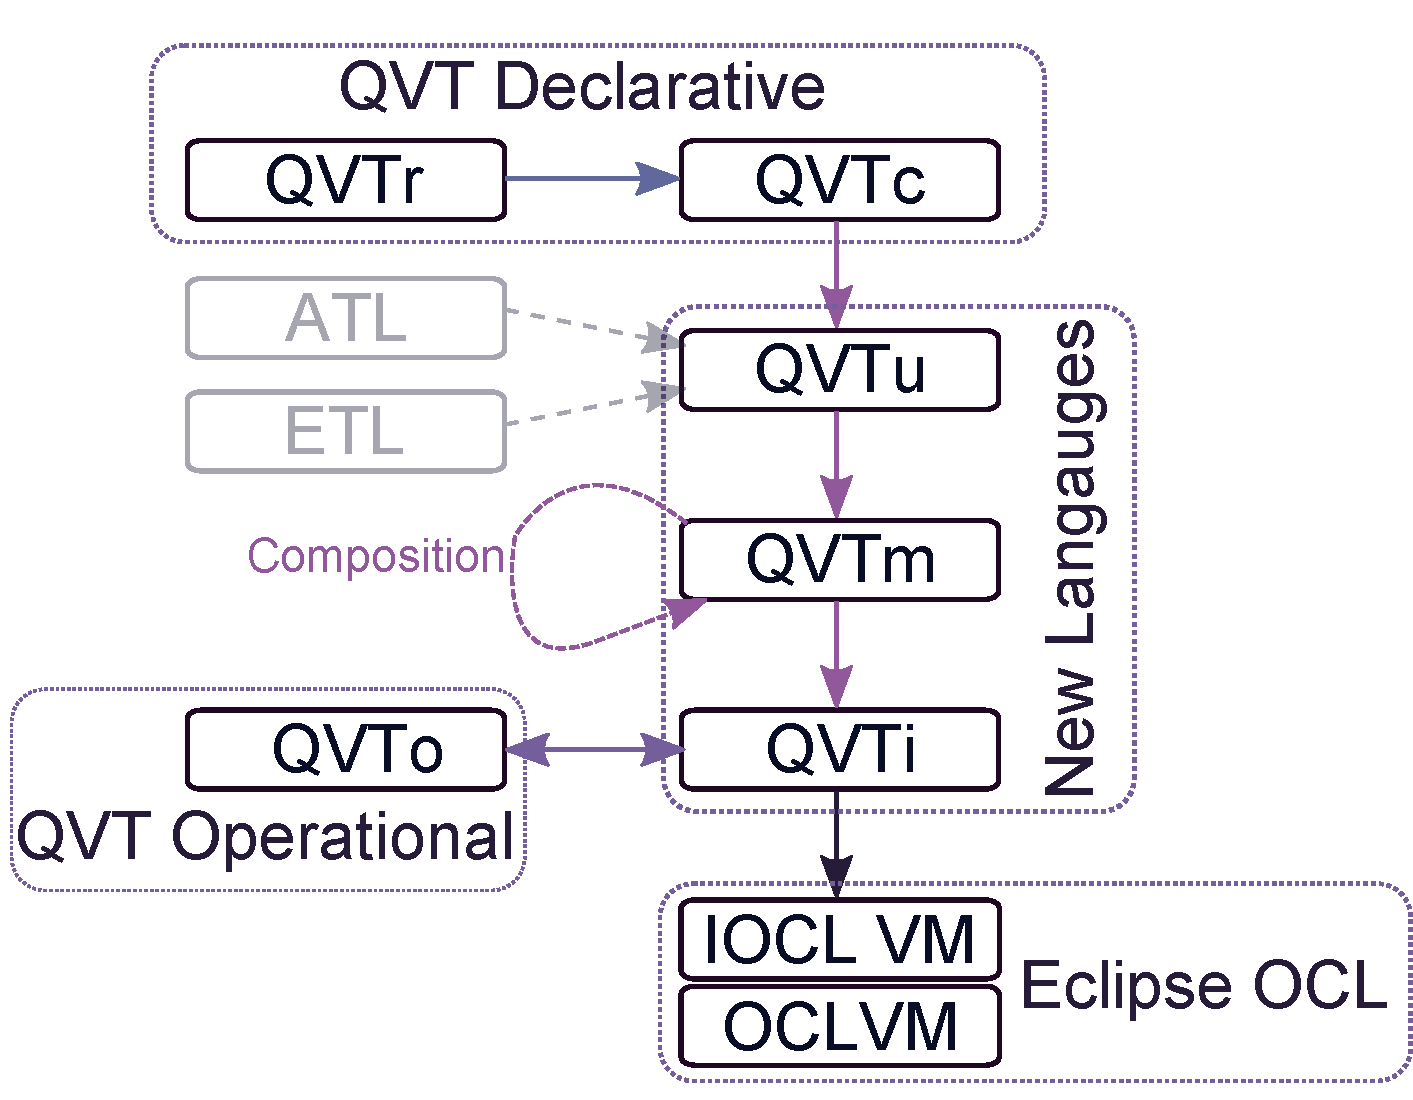
\includegraphics[width=0.56\textwidth]{QVTView.pdf}
	\caption{Overview of the proposed QVT 6 languages architecture.}
	\label{fig:overview}
\end{figure}

Figure \ref{fig:overview} presents our progressive transformation solution to realizing QVTr on an OCL Virtual Machine\cite{Willink2012}. At the top we have the two QVT Declarative languages, with QVTr realized by a QVTr to QVTc program-to-program transformation. Our three new languages, QVTu, QVTm and QVTi are syntactic and semantic simplifications of QVTc.

\begin{itemize}
\item For QVT Uni-directional (QVTu), we align the transformation to the user's invocation context and eliminate the redundant multi-directional and enforcement flexibilities.
\item For QVT Minimal (QVTm) we normalize to eliminate syntactic sugar and alternate representation flexibilities.
\item For QVT Imperative (QVTi) we discard declarative flexibilities and synthesize a multi-pass imperative search schedule that can be executed easily by a model-friendly Virtual Machine.
\end{itemize}

These new languages are not just a convenience for realizing QVTc, they also offer important interchange points for other transformation technologies to exploit and so share the tool chain.

\begin{itemize}
\item QVTu provides a high level interchange point for other uni-directional declarative transformation languages such as ATL or ETL.
\item QVTm provides a normalized representation at which declarative transformation composition and optimisation can be applied.
\item QVTi provides a low level interchange point that imperative transformation languages such as QVTo, ALF or EOL may exploit.
\end{itemize}

%three new languages, each one supporting a more restricted QVTc abstract syntax and providing increasingly limited semantics. QVTo operations will be invoked at the QVTi level and QVTi will provide an interface for QVTo to populate the middle (trace) model. Proximity of the QVTc abstract syntax to EMOF and OCL will be useful as an AST interpretation and execution can be provided by extending the Eclipse OCL Virtual Machine\cite{Willink2012}.

%The intention of the QVTc subset languages is then to progressively restrict the QVTc semantics to eventually define a subset of QVTc that is uni-directional, normalized and imperative. The different levels of semantic \textquotedblleft power\textquotedblright will also imply a restriction on the use of the language's abstract syntax, from permissive to restricted. An overview of the proposed QVT alphabet is presented in Figure \ref{fig:overview}. 

%Complete support for QVTr is achieved by specifying mappings and implementing automated program transformations for:
%\begin{itemize}
%\item  QVTr$\rightarrow$QVTc, written in QVTc
%\item  QVTc$\rightarrow$QVTu, written in QVTu
%\item  QVTu$\rightarrow$QVTm, written in QVTm
%\item  QVTm$\rightarrow$QVTi, written in QVTi
%\end{itemize}

%The first restriction is to remove bi-directionality, thus QVTu (unidirectional) restricts the semantics so that in the context of a mapping (the name given to rules in QVTc) only one candidate model can be enforced. The next restriction is to remove rule specialization, thus QVTm (minimal) does not allow mapping refinement. Finally, to remove the declarative component, in QVTi (imperative) mappings are allowed to introduce only one unbound variable and transformations must be written as a tree of mapping compositions were each root mapping declares the constraints between one of the candidate models and the trace model.  Execution of all the languages is provided by performing automated transformations from semantically richer languages to simpler ones, for example form QVTr to QVTc or from QVTm to QVTi.






